\chapter{Chaos}
\label{chap:chaos}

In this chapter, we will introduce the necessary mathematical theory and concepts from chaos theory that we will work with and that are relevant for this thesis.

\section{Outcome basin}
In dynamical systems, the concept of attractor can be described as a subset of a phase space toward which a system tends to evolve. An attractor's basin of attraction is the subset of the phase space such that any point (any initial condition) in that region will asymptotically evolve into the attractor. In the dynamical system of a black hole with a ring,
the test particle can evolve towards collision with the black hole or with the ring, escape to infinity or eternal orbit. An evolution towards eternal orbit or escape to infinity does not really satisfy the concept of an attractor. In order to capture and examine this behavior, we need to define what we will refer to as an outcome basin. 

\begin{defn}[Outcome basin]
An outcome basin is the set of initial conditions, i.e. a subset of the phase space, that evolve towards a given outcome.
\end{defn}

In our case, by outcome we understand eternal orbit, collision with a black hole or a ring, and escape to infinity.

\section{Basin boundary}
Let us now consider a specific system that has only two outcomes, hence two outcome basins. Denote the basin of the collision outcome by $C$ and $O$ as the basin of the eternal orbit outcome. By the boundary of these basins we understand the following:

\begin{defn}[Basin boundary]
Let \(O\) and \(C\) be two outcome basins. The subset \(\Sigma\) of the phase space that separates these two basins is called a basin boundary.
\end{defn}

If the dynamics of the system is regular (not chaotic), the basin boundary is
smooth. However, if the dynamics of the system is chaotic, therefore, sensitive to initial conditions, 
the basin boundary has fractal character.

\section{Fractals}
A fractal is a geometric shape that exhibits a self-similar pattern. A mathematical way of capturing this phenomenon of self-similarity and "roughness" of geometrical shapes is to use the concept of fractal dimension, which is a generalization
of a standard idea of dimension. The Hausdorff dimension $\dim_{\operatorname{H}}(X)$ of $X$ is defined by

\[
\dim_{\mathrm H}(X)
\coloneqq
\inf\left\{
d \geq 0 \,\middle|\, \mathcal{H}^{d}(X)=0
\right\}.
\]
For an introduction to fractal dimensions in the context of chaotic dynamics, see Ott~\cite{Ott2002}.

However, this is not the only definition of a fractal dimension. Another useful definition is the box-counting definition, also known as the Minkowski dimension.

\begin{defn}[Box-counting dimension]
Let \(S \subset \mathbb{R}^n\) be a bounded set and let
\(N(\varepsilon)\) denote the minimum number of n-dimensional boxes of side length
\(\varepsilon\) required to cover \(S\). The Minkowski
dimension, also called the box-counting dimension, is defined by
\[
d \equiv \dim_{\mathrm{B}}(S)
\coloneqq
\lim_{\varepsilon \to 0}
\frac{\ln N(\varepsilon)}
     {\ln(1/\varepsilon)},
\]
provided that the limit exists.
\end{defn}

Roughly speaking, this means that the number $N$ of n-dimensional boxes of size $\varepsilon$ covering the shape increases as we scale the size of the box down and this increase is proportional to $\left( \frac{1}{\varepsilon}\right)^d$. So we can write $N(\varepsilon)=C \left( \frac{1}{\varepsilon}\right)^d$.

Once we have established the concept of a fractal dimension, we can define fractals as geometric shapes that have a fractal dimension higher than the topological dimension.

\section{Uncertainty exponent}
\label{sec:uncertainty-exponent}
Suppose that we perturb a random initial condition by a small amount, 
$\varepsilon$, in a random direction. If the new trajectory ends up in a different basin from the unperturbed one, then the initial condition is called $\varepsilon$-uncertain.

\begin{figure}[H]
    \centering
    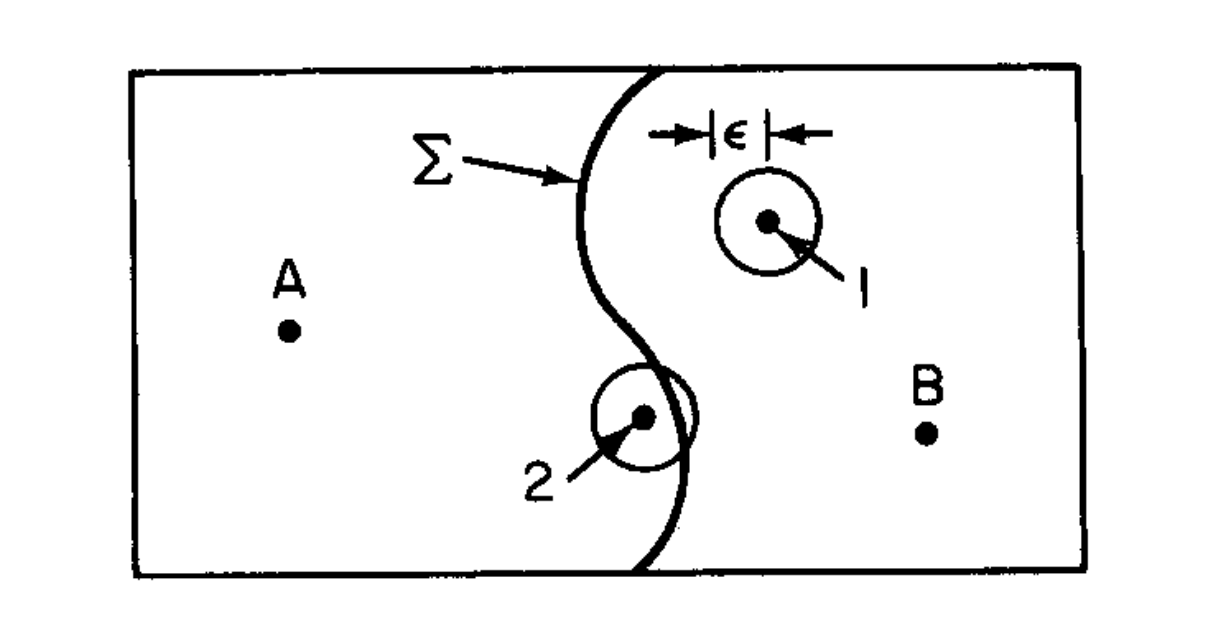
\includegraphics[width=0.72\linewidth]{img/region.png}
    \caption{Schematic region of phase space divided by a basin boundary into two basins of attraction. Initial conditions 1 and 2 illustrate the effect of uncertainty \(\varepsilon\) near the basin boundary. Adapted from Grebogi et al.~\cite{Grebogi1983}.}
    \label{fig:uncertain-initial-conditions}
\end{figure}

If we denote $\Omega$ a subset of a phase space in which we are interested and $U_{\varepsilon} \subset \Omega$ the set of uncertain initial conditions, we can define a ratio $f(\varepsilon) := \frac{Vol(U_{\varepsilon})}{Vol(\Omega)}$.
Then let us define a value $\alpha \coloneqq n-d$, where $n$ is the dimension of the phase space and $d$ is the box counting dimension of the basin boundary.
Following the uncertainty-exponent argument described by Grebogi et al.~\cite{Grebogi1983} and Ott~\cite[p.~206]{Ott2002},

\begin{equation}
  \bar{f} \sim \epsilon^{\alpha}.  
  \label{eq:uncertainty-scaling}
\end{equation}

Thus, we will refer to the value $\alpha$ as the uncertainty exponent. We can also rewrite \eqref{eq:uncertainty-scaling} as

\begin{equation}
    \ln{\bar{f}} = \ln{k} + \alpha\ln{\varepsilon}.
    \label{eq:uncertainty-log-fit}
\end{equation}

This form will be very useful in practice. Once we construct a basin map, we can select a smaller region of it. Consider an initial condition $(x_0,v_0)$. We can perturb the initial condition in the $x$ direction by some value $\varepsilon$, so we now have initial conditions $(x_0 + \varepsilon,v_0)$ and $(x_0 - \varepsilon,v_0)$. We check to which basin these new initial conditions correspond. If either of them does not correspond to the same basin as the original initial condition, we classify the original initial condition as uncertain. In this way, we perturb every initial condition in the smaller region and calculate how many of them are uncertain and denote this number by $N_U$. We define a ratio of the number of uncertain initial conditions to the total number of sampled initial conditions $N$ as $\bar{f}(\varepsilon):= \frac{N_U}{N}$. This fraction can be interpreted as the probability that a point chosen from the sampled region is uncertain. As the number of sampled points increases and the discretization becomes finer, $\bar{f}(\varepsilon)$ approaches $f(\varepsilon)$. When we repeat this process for more values of $\varepsilon$, we can perform a linear fit based on \eqref{eq:uncertainty-log-fit} to obtain the uncertainty exponent \(\alpha\). The fractal dimension of the basin boundary is then given by \(d=n-\alpha\).
